\section{Anwendung der Methodik auf die theoretischen Grundlagen}

\subsection{Prototypische Implementierung der Integrations- und Bereitstellungs-Pipelines}
\subsection{Evaluation der Integrations- und Bereitstellungs-Pipelines unter Anwendung des Analytischen Hierarchieprozesses}
\label{sec:AHP}
Als Entscheidungsalternativen werden CI/CD-Pipelines für die Bereitstellung von Cloud-Software gegenübergestellt. Konkret handelt es sich dabei, um die Tools \textit{SAP CI/CD}, \textit{Jenkins}, sowie \textit{Azure Pipelines}. Die Gegenüberstellung wird auf die genannten CI/CD-Pipelines beschränkt, da diese von der SAP als Best Practice definiert wurden. Bei der Untersuchung der Pipelines sind dabei verschiedene Aspekte zu beachten. So soll im Rahmen der Arbeit evaluiert werden, ob sich die verschiedenen Pipelines zur Bereitstellung von Software für CEs eignet. Darüber hinaus muss festgestellt werden, inwiefern die Tools für die Technologien SAP CAP bzw. SAP UI5 geeignet sind und ob eine Bereitstellung in der Laufzeitumgebung Cloud Foundry der SAP BTP möglich ist. 
\subsubsection{Festlegung der AHP-Entscheidungsalternativen}
 Die zur Durchführung des AHP-Verfahrens benötigten Daten werden neben einer Literaturrecherche ebenfalls mittels Experteninterviews erhoben. Dabei wird eine Expertengruppe aus X Mitarbeitenden der SAP zusammengestellt. Diese sind jeweils in spezifischen Bereichen der Cloud-Fullstack-Entwicklung, Test-Management, sowie im DevOps spezialisiert. Somit kann Expertise über verschiedene Fachbereiche hinweg aufgebaut und Anforderungen aller an der Entwicklung, Bereitstellung sowie den Betrieb von Software beteiligten Stakeholdern erfasst werden. Zur Festlegung der Entscheidungskriterien wird eine induktive Kodierung der Expertengespräche durchgeführt. Dabei werden aus besonders häufig von Experten genannten Aspekten systematisch Kategorien abgeleitet. Diese umfassen insbesondere Aspekte, welche die in vergangenen Entwicklungsprojekten hervorgegangenen Anforderungen an eine CI/CD-Pipeline darstellen. Da innerhalb dieser Kundenprojekte oft weniger strikte Qualitätsanforderungen an den CI/CD-Prozess gestellt werden, wird darüber hinaus erarbeitet, welche internen Bestimmungen von der SAP zur Bereitstellung von Standardsoftware definiert werden. Die bei der induktiven Kodierung erhobenen Kategorien werden anschließend ebenfalls als Entscheidungskriterien im AHP-Verfahren wiederverwendet. Die mit dieser Vorgehensweise erhobenen Entscheidungsalternativen sind folgender Abbildung zu entnehmen:
 \begin{center}
	\begin{figure}[H]
		\centering
		\scalebox{0.5}{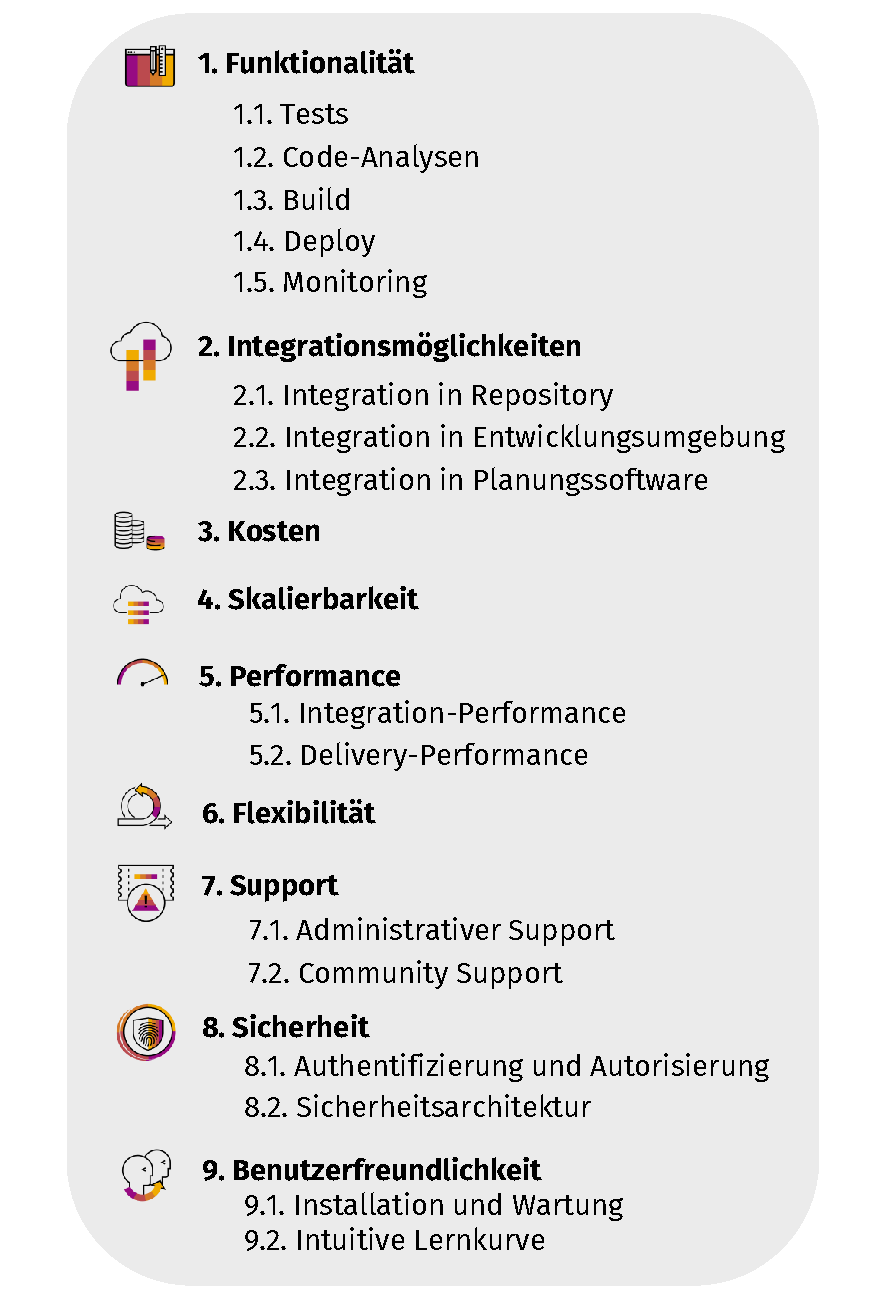
\includegraphics{AHP_E}}
		\caption[AHP-Entscheidungsstruktur zur Bewertung von CI/CD-Pipelines]{AHP-Entscheidungsstruktur zur Bewertung von CI/CD-Pipelines. Eigene Darstellung.}
		\label{fig:AHP_E}
	\end{figure}
\end{center}
\vspace*{-10mm}
 Auf der obersten Ebene des AHP-Entscheidungsbaums werden neun Kategorien definiert. Das erste Kriterium ist \textbf{Funktionalität} (K1). Diese Kategorie umfasst verschiedene innerhalb des CI/CD-Workflows benötigte funktionale Spezifikationen. So sollte eine Pipeline etwa dazu in der Lage sein, Anwendungen zu testen, Code-Analysen durchzuführen und eine Software auf der Cloud-Plattform bereitzustellen. Experte 1 begründet dabei, dass es \enquote{eine Unterstützung dieser Stufen benötigt, um eine effiziente Bereitstellung von Software zu ermöglichen.} Angesichts der Vielfältigkeit des Entscheidungskriteriums Funktionalität, wird eine Untergliederung in verschiedene Subkriterien vorgenommen. In Kategorie 1.1 wird evaluiert, welche Tests von der Pipeline unterstützt werden. Von der SAP werden diesbezüglich Produktstandards vorgegeben. Diese stützen sich auf \textit{ISO 9001}, eine internationale Norm für Qualitätsstandards. Im Kontext der Softwareentwicklung verlangt diese, eine für neue Funktionalität kontinuierliche und automatisierte durchgeführte Prüfung. Hinsichtlich der Entwicklung von CAP-Node-Anwendungen schreibt die SAP in ihren Produktstandards die Durchführung von Unit-Tests mittels Jest bzw. Mocha und Integration-Tests sowie Functional-Tests mittels Newmann vor. Für die Programmierung mit SAP UI5 sind hingegen Unit-Tests mittels Q-Unit, Integration sowie Functional-Tests mittels OPA5 und E2E-Tests mittels WDI5 vorgesehen. Während die Test-Frameworks Jest, Mocha, Newmann sowie Q-Unit in einer herkömmlichen Node-Laufzeitumgebung ausgeführt werden, benötigt es für OPA5 sowie WDI5 einer emulierten Browser-Umgebung. Die von dem Emulator generierte Benutzeroberfläche ermöglicht das Simulieren und Testen von gezielten Anwenderinteraktionen. Diese können z.B. das Ausfüllen von Formularen bzw. das Klicken auf Schaltflächen darstellen. Bei der Bewertung soll deshalb insbesondere evaluiert werden, ob neben der Node-Laufzeitumgebung ebenfalls eine emulierte Browser-Umgebung von den zu vergleichenden Pipelines unterstützt wird.\\ 
In Kriterium K1.2 wird die Kompatibilität verschiedener \textit{Code-Analyse-Tools} untersucht. Es wurde gezielt eine Trennung dieser Kategorie mit dem Kriterium K1.2 (Tests) vorgenommen. Während Tests eine funktionale Erfüllung der Anforderung evaluieren werden mit Code-Analysen Code-Qualitätsstandards der entwickelten Features untersucht. Dabei wird evaluiert, ob statische Codeanalysen, Security- sowie Performance-Überprüfungen von den CI/CD-Pipelines unterstützt werden. Gemäß den Produktstandards der SAP sind für statische Code-Analysen Lint sowie SonarQube vorgeschrieben. Mit diesen Tools können neben syntaktischen Formqualitätsüberprüfungen ebenfalls Code-Metriken wie Komplexität oder Quellcode-Duplikate analysiert werden. Zur Durchführung von Sicherheitsüberprüfungen wird bei SAP CAP-Node-Anwendungen Checkmarx verwendet, während bei SAP UI5 DASTER zum Einsatz kommt. Die Unterstützung solcher Sicherheits-Tools ist dabei insbesondere für eine CEA essenziell. Die Verwendung von APIs zur Kommunikation zwischen einzelnen Microservices hat zur Folge, dass eine für unautorisierte Zugriffe begünstigte Angriffsfläche entsteht. Während für Performance-Tests von der SAP das Tool JMeter vorgeschlagen wird, gibt es bezüglich der Code-Coverage-Checks keine spezifische Vorgabe.\\
In der Kategorie K1.3 werden die \textit{Build-Funktionalitäten} der CI/CD-Pipelines evaluiert. 
Um Anwendungen in die Cloud Foundry Laufzeitumgebung der SAP BTP bereitzustellen wird i.d.R. das Mulit-Target-Application-Konzept (MTA-Konzept) verwendet.
\begin{center}
	\begin{figure}[H]
		\centering
		\scalebox{0.25}{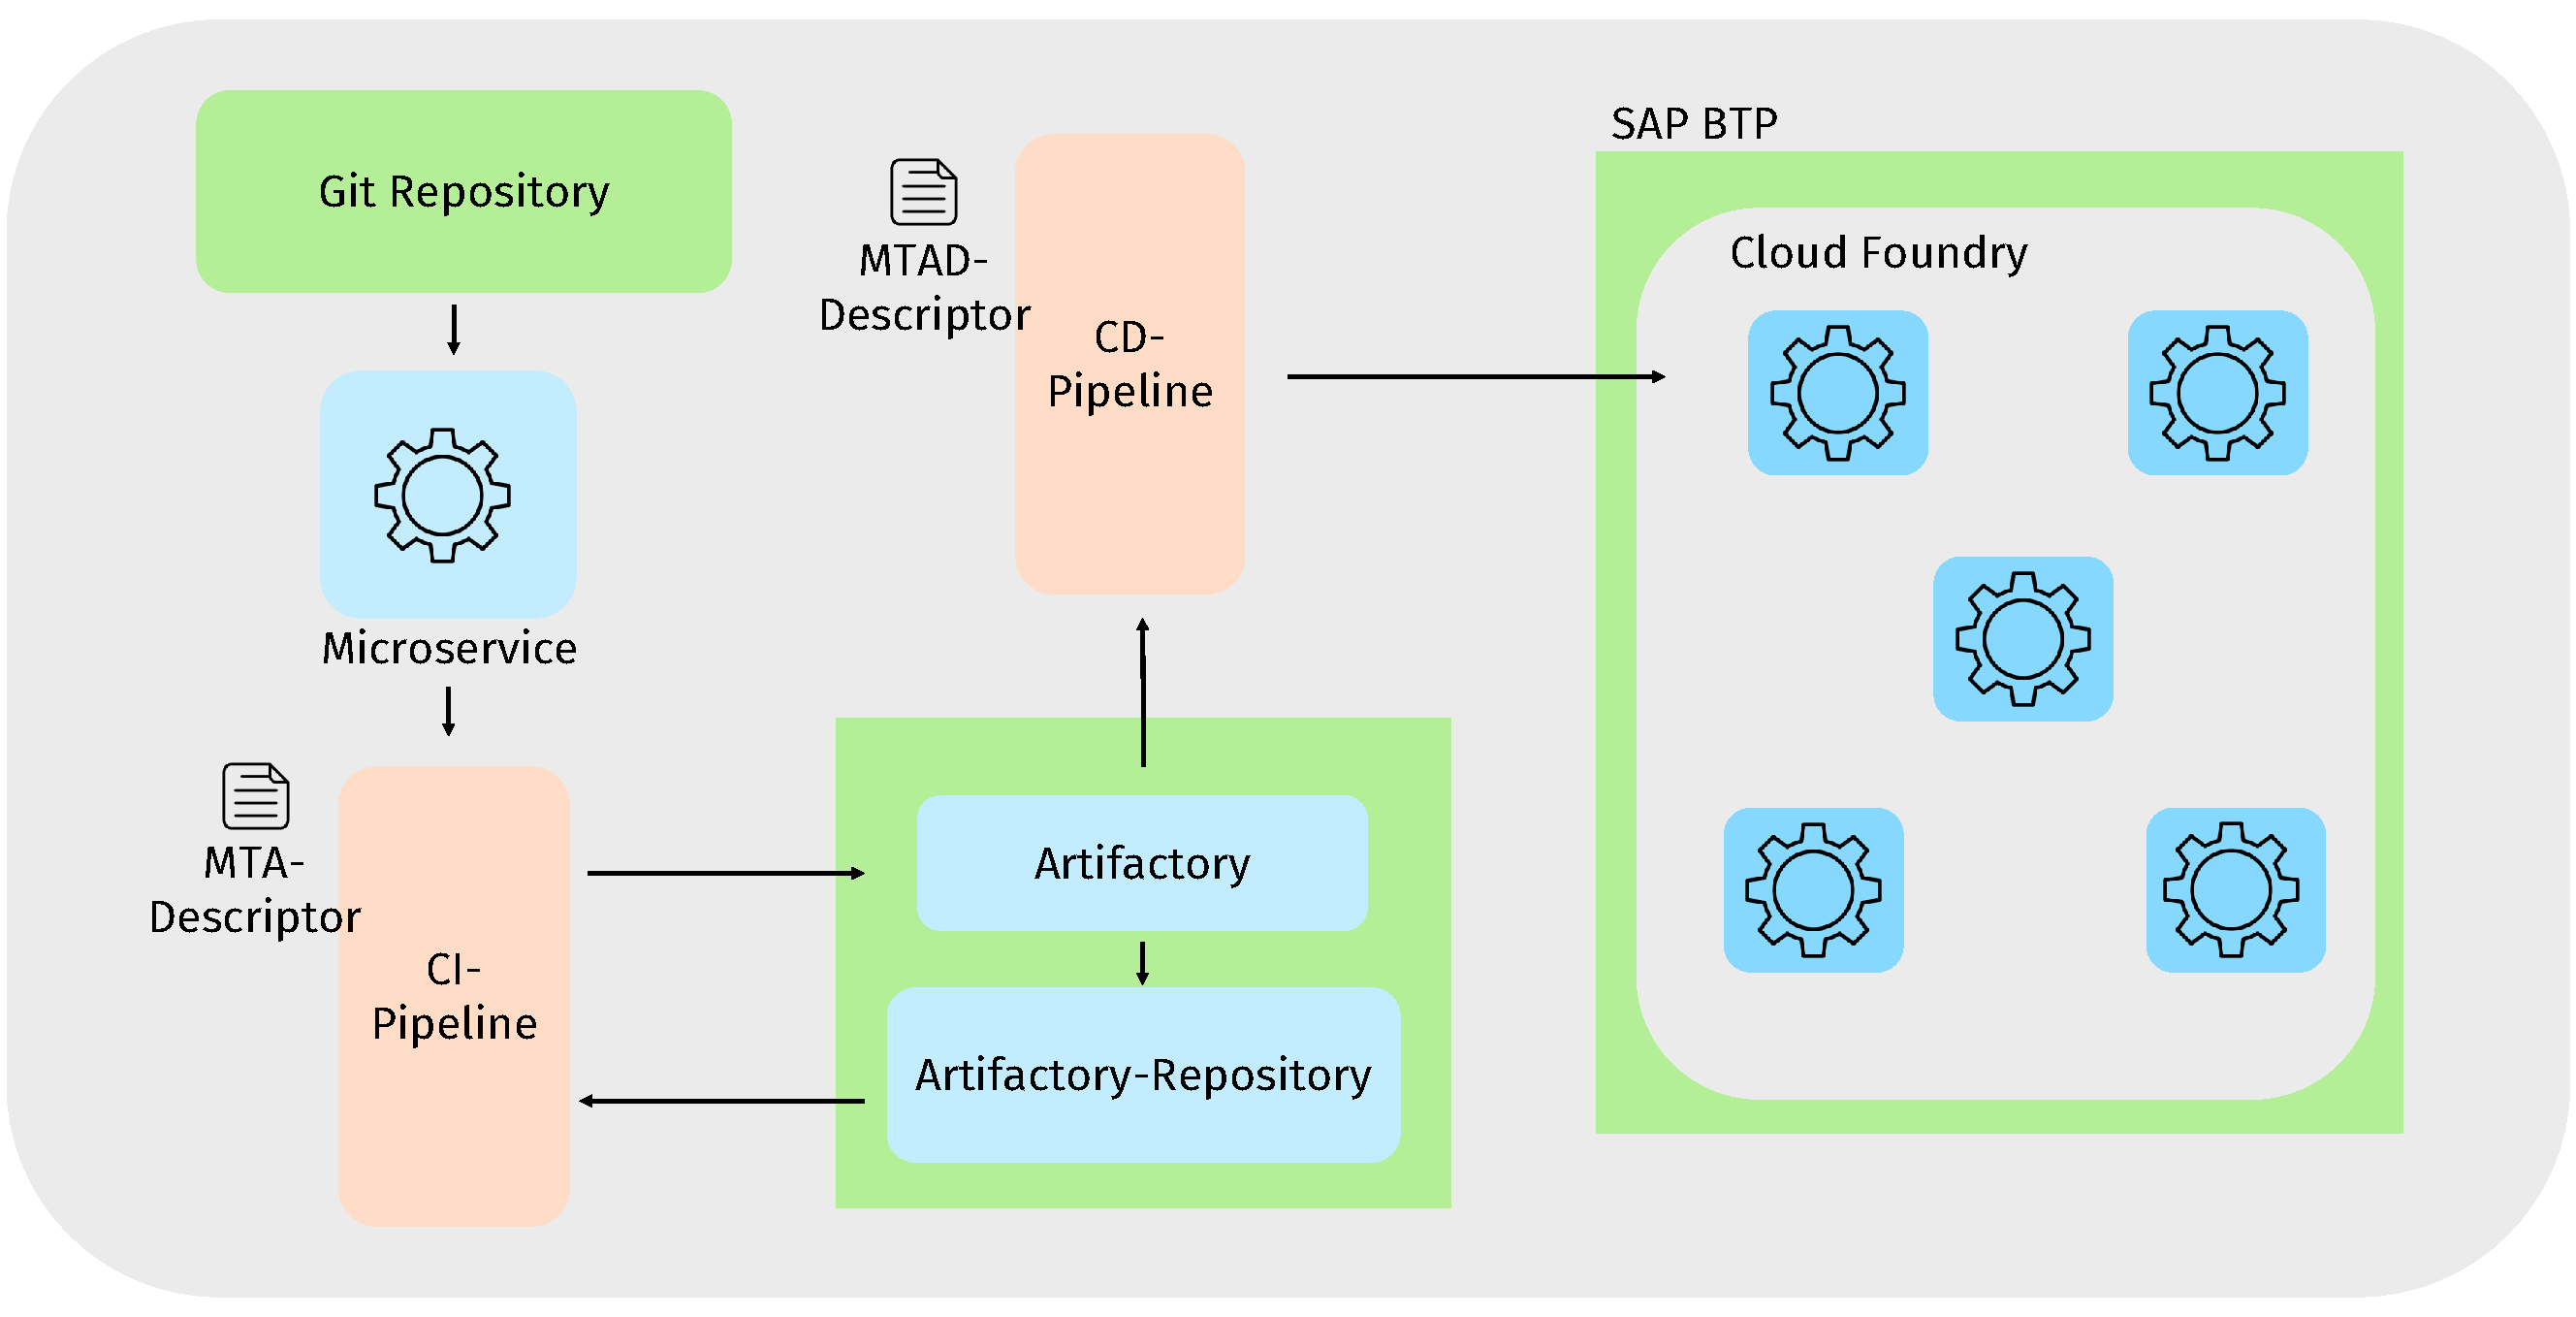
\includegraphics{MTA}}
		\caption[Bereitstellung von MTA-Applikationen in ein Artefakt-Repository]{Bereitstellung von MTA-Applikationen in ein Artefakt-Repository. Eigene Darstellung.}
		\label{fig:MTA}
	\end{figure}
\end{center}
\vspace*{-10mm}
Die MTA ist eine Applikation, z.B. ein Microservice eines CEs, welche aus verschiedenen Modulen besteht. Diese Module umfassen typischerweise die durch einen Microservice bereitgestellte API oder eine von der Applikation verwendete Datenbank sein. Eine CE-Anwendung kann dabei ebenfalls von verschiedenen externen Ressourcen abhängig sein. Diese sind in einem Artefakt-Repository verwaltete externe Komponenten, welche bei der Entwicklung neuer Microservices wiederverwendet werden können. Diese Komponenten werden während des Build-Prozesses von der CI/CD-Pipeline aus den Artefakt-Repositorys geladen. Darüber hinaus können die von einer CI/CD-Pipeline bereitgestellten Anwendungen ebenfalls als wiederverwendbare Komponenten in das  Artefakt-Repository eingelagert werden. Für CEA ist vorteilhaft, wenn verwendete CI/CD-Pipelines Docker-Workflows unterstützen. Durch den Einsatz von Docker-Containern können Entwickler schnell virtualisierte Umgebungen mit benötigten Frameworks und Tools bereitstellen ohne dabei eine gesamte Infrastruktur manuell konfigurieren zu müssen. Innerhalb dieses Bewertungskriteriums wird deshalb evaluiert ob, Build-Tools für MTA, Artefakt-Repositorys sowie Docker-Workflows durch die CI/CD-Pipelines unterstützt werden.\\
In Kriterium K1.4 werden die \textit{Deploy- und Release-Prozesse} der CI/CD-Tools untersucht. Dabei wird evaluiert, ob die Pipelines verschiedene Bereitstellungsstrategien (z.B. Blue/Green-Deployment s. Kap. \ref{sec:Bereitstellungs_Strategien}) unterstützen. Diese Strategien gewährleisten die notwendige Flexibilität und Agilität, welche es in CEs benötigt. Auf diese Weise können neue Anwendungsversionen schnell und ohne Beeinträchtigung der Produktivsysteme bereitgestellt und getestet werden. Des Weiteren wird erörtert, ob die CI/CD-Pipelines eine Bereitstellung in das \ac{SAP CTM} unterstützten.
\begin{center}
	\begin{figure}[H]
		\centering
		\scalebox{0.3}{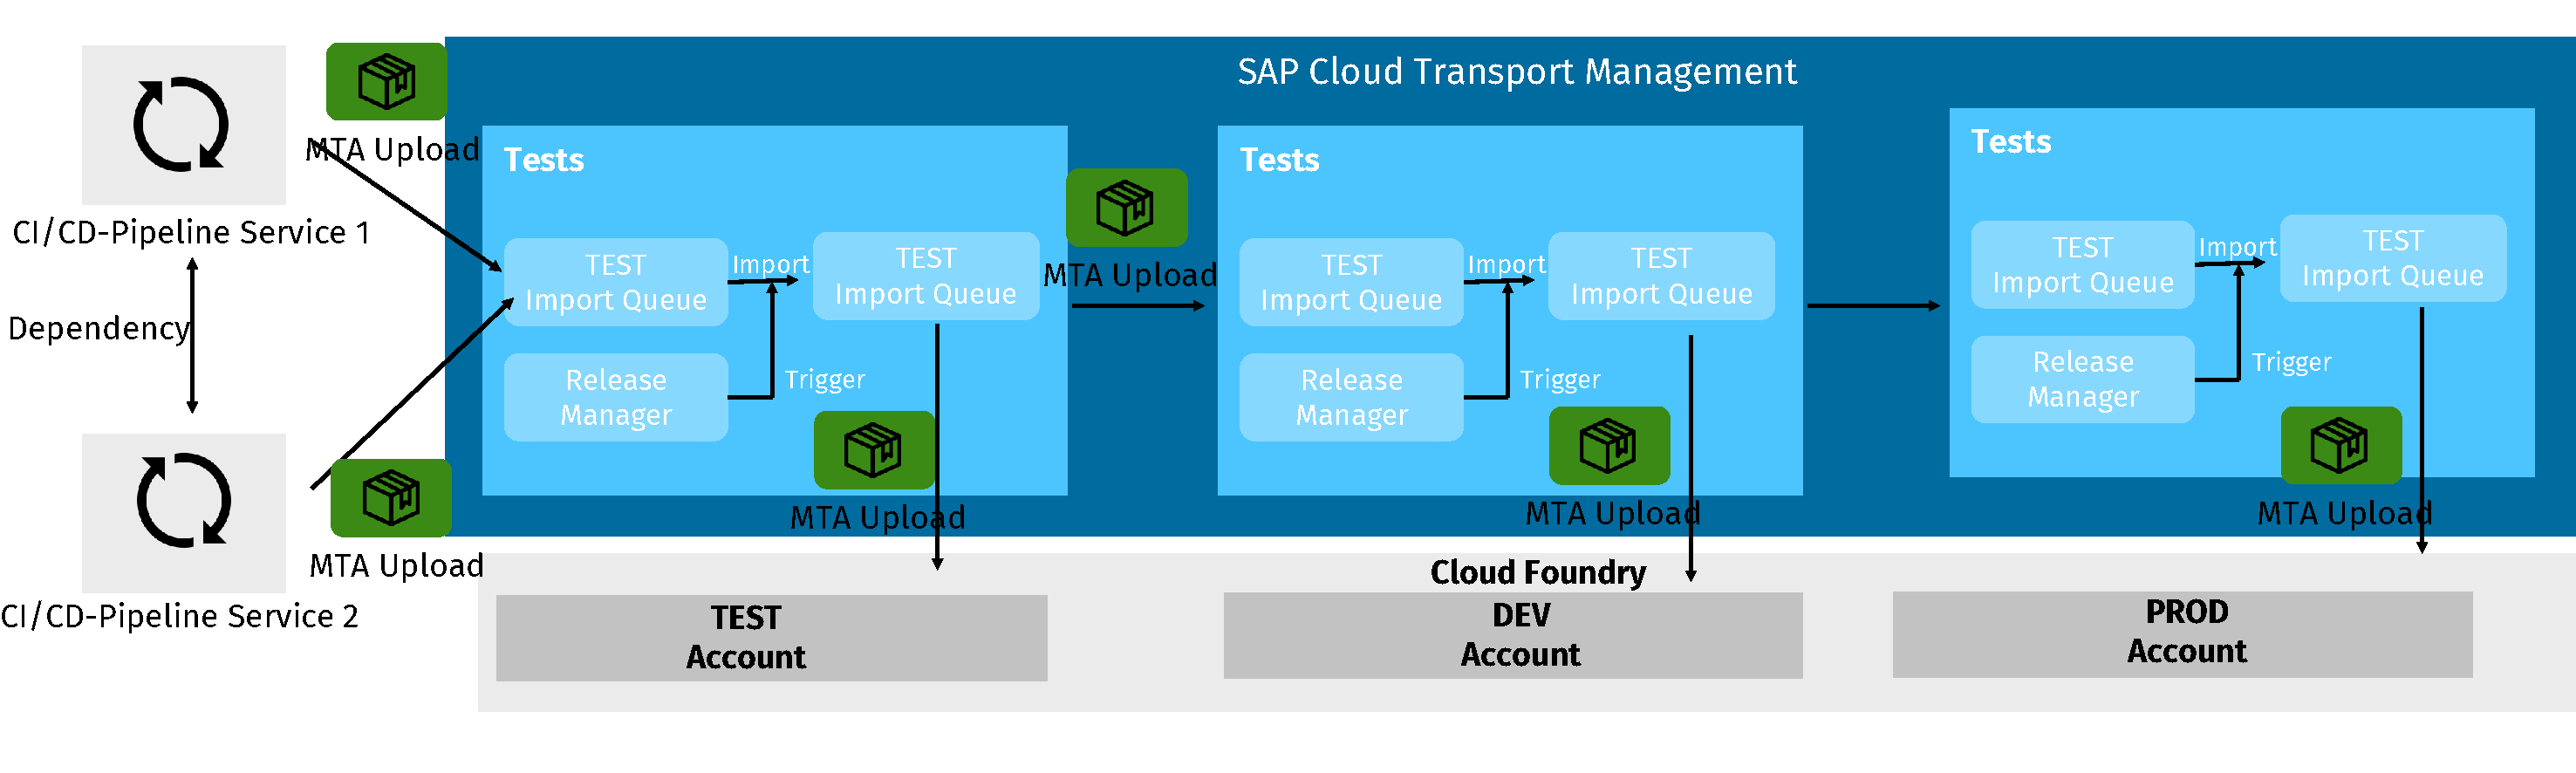
\includegraphics{CTM}}
		\caption[SAP Cloud Transportmanagement]{SAP Cloud Transportmanagement. Eigene Darstellung.}
		\label{fig:CTM}
	\end{figure}
\end{center}
\vspace*{-10mm}
Das SAP CTM kann als zusätzliche Schicht im CI/CD-Prozess verbaut werden (s. Abb. \ref{fig:CTM}). Mit dem SAP CTM können Anwendungsartefakte zwischen verschiedenen Accounts der SAP BTP verschoben werden. So könnte ein Unternehmen etwa einen Account für das Testen (TEST) bzw. für die Produktionsumgebung (PROD) besitzen. Nachdem der Entwickler seine Funktionalitäten fertiggestellt hat, kann das entsprechende Artefakt für letzte die manuellen Tests der Qualitätssicherung unmittelbar in die TEST-Umgebung bereitgestellt werden. Die Bereitstellung in die PROD-Umgebung erfolgt dabei unter Verwendung des SAP CTM durch das Betriebsteam. Dabei stellt das SAP CTM diverse Funktionalitäten, darunter eine eine zeitplangesteuerte Bereitstellung sowie das Definieren von Abhängigkeiten zu anderen Microservices, bereit.  
In Kategorie K1.5 wird die \textit{Monitoring-Funktionalität} der verschiedenen CI/CD-Pipelines untersucht. In diesem Zusammenhang erfolgt eine Bewertung der Überwachbarkeit der CI/CD-Tools. So soll der fehlerfreie Bereitstellungs-Workflow etwa anhand von Logs oder Metriken wie Build-Zeiten evaluiert werden. Zusätzlich sollte es möglich sein, die Abwicklung der Tests sowie die Bereitstellung in die Produktionsumgebung zu überwachen.\\
In Kategorie K2 werden die \textbf{Integrationsmöglichkeiten} der Pipeline untersucht. In dem Subkriterium \textit{Integrationsmöglichkeiten von Repositorys} (Kriterium K2.1) wird evaluiert, ob sich das Repository in die Pipeline integrieren lässt. Dies ist beispielsweise über Webhooks möglich. Mit diesen können bestimmte Ereignisse, wie das Pushen von Code-Änderungen in einem Repository automatisch an die CI/CD-Pipeline gesendet werden. Somit kann ein unmittelbarer Integrations- bzw. Bereitstellungs-Workflow ausgelöst werden. Bei der Bewertung wird dabei insbesondere darauf geachtet, dass häufig verwendete Repositorys in die Pipeline integrierbar sind. In Kriterium K1.2 werden die \textit{Integrationsmöglichkeiten von Entwicklungsumgebung} untersucht. Die Integration-Pipeline kann unmittelbar während des Entwicklungsprozesses aus der Entwicklungsumgebung gestartet werden. Auf diese Weise wird sichergestellt, dass Entwickler Feedback in noch kürzerer Zeit erhalten als bei einer ausschließlichen Integration der Pipeline in das Repository. Die Bewertung bezieht sich dabei ausschließlich auf SAP UI5 sowie SAP CAP Entwicklungsumgebungen. Dazu gehören Microsoft Visual Studio Code, \ac{SAP BAS} sowie Eclipse.
In Kriterium K2.3 wird die \textit{Integrationsmöglichkeiten von Planungssoftware} untersucht. Dazu gehören Projektmanagement-Tools wie Jira. Eine Integration solcher Planungssoftware erlaubt Projektmanager eine erhöhte Transparenz über den Bereitstellungs-Workflow aller zu implementierender Arbeitselemente zu erlangen. Auf diese Weise kann der CI/CD-Status eines Backlog-Items unmittelbar über die Planungssoftware eingesehen werden. Da keine SAP-spezifischen Vorgaben bezüglich Planungssoftware getroffen sind, erfolgt lediglich eine Untersuchung der generellen Integrationsfähigkeit von Planungssoftware.\\ 
In Kriterium K3 erfolgt die Evaluation der \textbf{Kosten}. Um eine Vergleichbarkeit herzustellen, wird eine Analyse der Kosten pro Build-Stunde durchgeführt. Da die Installation und Wartung von Jenkins auf einem eigenen Server mit zusätzlichen Kosten verbunden ist, wird eine Bewertung der Kosten für eine in der Cloud betriebene Jenkins-Instanz durchgeführt. Hierfür wird der von SAP Hyperspace verwaltete \ac{JaaS} als Vergleichsgrundlage verwendet.\\
Das Kriterium K4 untersucht die \textit{Skalierbarkeit} der CI/CD-Pipelines. Hierbei werden die Pipelines auf horizontale so wie vertikale Skalierbarkeit untersucht. Die horizontale Skalierbarkeit ermöglicht eine parallele Durchführung mehrerer Builds. Gerade bei einer hohen Anzahl gleichzeitiger Hauptzweigintegrationen birgt dies einen hohen Mehrwert. Die vertikale Skalierung bezieht sich auf die Erhöhung der Ressourcen einer Pipeline-Instanz. So kann die CI/CD-Pipeline dynamisch an die sich ändernden Anforderungen eines angepasst werden. Insbesondere für  CEs kann dies einen hohen Mehrwert darstellen. Durch schnelle und effiziente Entwicklungs- und Bereitstellugnsprozesse können diese Unternehmen das Time-to-Market verkürzen und somit schneller auf die Bedürfnisse der Kunden reagieren.\\
In Kriterium K5 wird die \textit{Performance} der verschiedenen CI/CD-Pipeline verglichen. Dabei werden die zu untersuchenden Tools anhand derselben Anwendung getestet. Damit soll für jede Pipeline die zur Prozessierung des CI/CD-Workflows benötigte Zeit gemessen werden. Im Rahmen dieser Gegenüberstellung wird eine Unterscheidung zwischen der Integration- bzw. Delivery-Zeit realisiert. Die Integration-Zeit bezeichnet den Zeitraum, welcher von der Einführung eines Feature-Branchs bis zur vollständigen Konsolidierung in den Hauptzweig benötigt wird. Dabei werden in die Pipelines dem CI-Prozess entsprechende Validierungen wie Unit- und Integration-Tests eingebaut. Die Delivery-Zeit beschreibt die Zeitspanne, welche von der Freigabe des Hauptzweigs bis zur Bereitstellung der Software auf die Cloud-Plattform benötigt wird. Dabei werden CD-typische Schritte in die Pipelines integriert. Dazu gehört das Ausführen von Code-Analysen und E2E-Tests.\\
In Kriterium K6 wird die \textbf{Flexibilität} der verschiedenen Pipelines evaluiert. Eine bedeutende Dimension der Flexibilität ist die uneingeschränkte Konfigurierbarkeit der Pipelines. So sollte eine Pipeline etwa keinerlei Beschränkungen in Bezug auf Anzahl und Reihenfolge der im CI/CD-Workflow durchzuführenden Schritten besitzen. Weiterhin wird evaluiert, ob für die Pipeline ein modularer Aufbau möglich ist. Da CEs i.d.R. über eine Vielzahl an Services verfügen, bedarf es ebenfalls einer hohen Anzahl an Pipelines. Um die daraus resultierende Komplexität zu reduzieren, sollten Pipelines aus modularen wiederverwendbaren Komponenten bestehen. Wird ein neuer Service in die Systemlandschaft integriert, können diese Komponenten somit ohne hohen Aufwand wiederverwendet werden. Ein weiterer für die Flexibilität der Pipelines essenzieller Aspekt ist die Unterstützung von Plugins. Mit Plugins können ebenfalls nicht im Standard verfügbare Funktionen in die Pipeline integriert werden. Dadurch sind CEs in der Lage, agil auf sich ändernde Bedürfnisse zu reagieren  und können somit unabhängig von dem mit der Pipeline ausgelieferten Standard operieren.\\  
In Kriterium K7 wird der für die CI/CD-Pipelines bereitgestellte \textbf{Support} evaluiert. Hierfür werden die Subkriterien \textit{Administrativer Support} sowie \textit{Community-Support} gebildet. Im Hinblick auf den \textit{Administrativen Support} wird geprüft, ob die Pipeline-Anbieter Unterstützung bei der Einrichtung, Konfiguration sowie Problembehebung der CI/CD-Tools bietet. Dies ist insbesondere dann hilfreich, wenn der Umgang mit den Pipelines einen hohen Grad an Expertise benötigt. Des Weiteren wird evaluiert, ob Schulungen sowie Informationsmaterial verfügbar sind. Ein weiterer wesentlicher Aspekt ist die Verfügbarkeit von Updates. Durch kontinuierliche Updates kann sichergestellt werden, dass die Pipeline stets auf dem neusten Stand der Technik ist. Im Kontext des \textit{Community-Supports} wird geprüft, ob öffentliche Foren existieren, in welchen Anwender Fragen stellen und Probleme diskutieren können. Darüber hinaus wird evaluiert, inwiefern eine Community zur Erweiterung der Dokumentation oder zur Entwicklung neuer Funktionalität beiträgt.\\
In dem Kriterium K8 wird die \textbf{Sicherheit} der CI/CD-Pipelines untersucht. Hierbei werden die Subkriterien \textit{Authentifizierung und Autorisierung} bzw. \textit{Sicherheitsarchitektur} gebildet. Im Kontext der \textit{Authentifizierung und Autorisierung} wird evaluiert, ob eine CI/CD-Pipeline geeignete Sicherheitsmaßnahmen implementiert. Um unerwünschte Zugriffe zu vermeiden, sollte die Verwendung einer Pipeline ausschließlich über eine Nutzer-Passwort-Kennung möglich sein. Besonders vorteilhaft ist dabei die Einbindung zentralisierte Drittanbieter, wie der SAP Identity Provider oder GitHub. Damit kritische Konfiguration ausschließlich von Spezialisten vorgenommen werden, muss eine Pipeline ebenfalls Autentisierungskonzepte unterstützten. Dabei sollen Benutzern über die Implementierung von Rollen bestimmte Rechte eingeräumt werden können. Unter dem Aspekt der \textit{Sicherheitsarchitektur} wird die Systemintegrität der Pipeline-Tools untersucht. Zu Erhöhung der Sicherheit ist es z.B. vorteilhaft, wenn CI/CD-Pipelines in isolierten Umgebung, wie z.B. Docker-Container oder virtualisierten Maschinen laufen. Entstehen in der CI/CD-Pipeline Lücken, können sich diese nicht unmittelbar auf andere Systeme ausweiten. Ein weiterer in diesem Kriterium evaluierter Aspekt ist die Ausfallsicherheit. Um sicherzustellen, dass neue Funktionalität bei der Integration kontinuierlich getestet und Software schnell an den Kunden bereitgestellt werden kann, sollten die CI/CD-Systeme stets hochverfügbar sein.
In Kriterium K9 wird die \textbf{Benutzerfreundlichkeit} der CI/CD-Pipelines untersucht. Dafür wird eine Unterteilung in \textit{Installation und Wartung} sowie in \textit{Intuitive Bedienbarkeit} vorgenommen. Hinsichtlich des Kriteriums der \textit{Installation und Wartung} ist es dabei besonders vorteilhaft, wenn das CI/CD-Tool nicht installiert werden muss, sondern unmittelbar als Service bereitgestellt wird. Um sicherzustellen, dass die Pipeline hochverfügbar ist, sollte das Bereitstellungssystem kontinuierlich gewartet werden. Wird die Wartung dabei als Dienstleistung von einem CI/CD-Plattformanbieter übernommen, kann ein Unternehmen die Fachkraft auf das Kerngeschäft und somit auf die Entwicklung neuer Services konzentrieren. Auch der für die Implementierung und Konfiguration der Pipelines benötigte Aufwand sollte so gering wie möglich sein (\textit{intuitive Bedienbarkeit}). Um die Abhängigkeit einer Abteilung von hochqualifizierten DevOps-Spezialisten zu veringern, kann es etwa von Vorteil sein, wenn Pipelines nicht mittels Programmiersprachen, sondern über intuitive Benutzeroberfläche konfigurierbar sind.  
\subsection{Entwicklung einer ganzheitlichen Bereitstellungsstrategie}
 